% \chapter{Impact of CPython performance enhancements on xDSL pattern rewriting}
% \chapter{CPython optimizations' impact on xDSL pattern rewriting}
% \chapter{Impact of CPython Optimizations on xDSL Pattern Rewriting}
\chapter{CPython optimisations for xDSL}
\label{chap:impact-cpython-pattern-rewriting}

% Hook
\acf{pep} 659 asserts that ``Python is widely acknowledged as slow'' \cite{pep659}.
% Argument
This comes partially as an inherent trade-off from the benefits of its interpreted runtime and expressive dynamic semantics, meaning it cannot achieve the general-purpose performance of ahead-of-time compiled languages such as C++ or FORTRAN. However, it is feasible for Python implementations to be competitive with fast implementations of other scripting languages with similar trade-offs, such as JavaScript's V8 or Lua's LuaJIT. The Faster CPython project is an attempt to achieve this goal in Python's reference implementation. Over the course of the recent CPython major versions, new optimisations have been gradually added as part of this project, resulting in incremental performance gains (\autoref{tab:faster-cpython}).
% Link
This section discusses the details of these optimisations, and their effect on user-extensible compiler workloads in xDSL.


\section{Specialising adaptive interpreter}
\label{sec:specialising-adaptive-interpreter}

%% What is the idea?
% Hook
Simple interpreters of dynamic languages use generic instructions which can express functionality over a wide array of types. However, this incurs an overhead selecting the specific implementation for the current type at runtime.
% Argument
In 2009, Williams et al. introduced the concept of instruction specialisation in their paper ``Dynamic Interpretation for Dynamic Scripting Languages'' \cite{williamsDynamicInterpretationDynamic2010}.
This proposes a novel dynamic \ac{ir} for Lua, whose operations can be specialised to a more performant implementation based on types and control flow encountered at runtime, claiming an average speedup of $1.3\times$.
Following this, Mark Shannon applied the idea to the Python language in his doctoral thesis ``The construction of high-performance virtual
machines for dynamic languages'' \cite{shannonConstructionHighperformanceVirtual2011}, demonstrating its viability through the research \ac{vm} HotPy.
% Link
This idea was realised in the CPython through \ac{pep} 659's specialising adaptive interpreter, enabled by default in the 2022 minor version 3.11 release.

%% NOTE: Lifted later to pack pages more efficiently
\begin{table}[H]
  \caption{Incremental improvements of the geometric mean of speedups across the PyPerformance benchmark suite (full results \autoref{chap:pyperformance-version-comparison}), achieved by optimisations to the CPython interpreter since CPython 3.10.}
  \label{tab:faster-cpython}
  \centering
  \begin{tabular}{llrr}
    % \toprule
    % \multicolumn{2}{c}{\textbf{Python executable}} \\
    % \cmidrule(r){1-2}
    % \textbf{Implementation} & \textbf{Feature flags} & \textbf{PyPerformance speedup} \\
    % \midrule
    % CPython 3.10.17 & None & $1\times$ \\
    % CPython 3.11.12 & None & $1.257\times$ \\
    % CPython 3.13.3 & None & $1.312\times$ \\
    % CPython 3.13.3 & \texttt{--enable-experimental-jit} & $1.397\times$ \\
    % CPython 3.14.0a7 & None & $1\times$ \\
    % CPython 3.14.0a7 & Tail call interpreter & $1\times$ \\
    \toprule
    \multicolumn{2}{c}{\textbf{Python executable}} & \multicolumn{2}{c}{\textbf{PyPerformance speedup}}\\
    \cmidrule(r){1-2} \cmidrule(r){3-4}
    \textbf{Implementation} & \textbf{Feature flag} & \textbf{Baseline} & \textbf{Previous} \\
    \midrule
    CPython 3.10.17 & None & $1\times$ & $1\times$ \\
    CPython 3.11.12 & None & $1.241\times$ & $1.241\times$ \\
    CPython 3.13.3 & None & $1.312\times$ & $1.078\times$ \\
    CPython 3.13.3 & Experimental JIT & $1.295\times$ & $0.988\times$ \\
    \bottomrule
  \end{tabular}
\end{table}

%% How is it implemented?
% Hook
The specialising adaptive interpreter implements this by replacing instructions which can be optimised by specialisation, such as the generic \texttt{LOAD\_ATTR}, with an adaptive form, such as \texttt{LOAD\_ATTR\_ADAPTIVE}. Each adaptive instruction maintains an internal counter, incrementing it when the observed usage matches a specialisation opportunity, and decrementing when it does not. When this counter exceeds a threshold, the adaptive instruction replaces itself with the appropriate specialised version, in a process known as a quickening. For example \texttt{LOAD\_ATTR\_ADAPTIVE} becomes \texttt{LOAD\_ATTR\_INSTANCE\_VALUE} when the attribute is an instance of the class for previous execution paths of the instruction.
If the assumptions required for specialisation are violated later, then the interpreter can fall back to the original instruction implementation to ensure correctness.
The optimisation is transparent to users, as no code changes are required, and the interpreter ensures correctness through its fall-back mechanism.
The specialising adaptive interpreter's documentation claims a speedup of $10\%$ -- $60\%$ \cite{pep659}, matching our recorded geometric mean improvement of $24\%$ for the PyPerformance benchmarks (\autoref{tab:faster-cpython}).
% Of these benchmarks, the one with the greatest improvement is \texttt{scimark\_monte\_carlo}, with a $66\%$ speedup. The implementation of this benchmark
% \footnote{\scriptsize{\url{https://github.com/python/pyperformance/blob/ec9e29/.../bm_scimark/run\_benchmark.py\#L201}}}
% Link
This is substantiated by an ablation of the feature across the previously discussed real-world workload and micro-benchmarks.


\begin{table}[H]
  \caption{Execution time per operation improves by a geometric mean speedup of $1.36\times$ across micro-benchmarks and real-world workloads in xDSL when the specialising adaptive interpreter is used (CPython 3.11).}
  \label{tab:specialising-adaptive-interpreter-xdsl}
  \centering
  \begin{tabular}{lrrr}
    \toprule
    & \multicolumn{2}{c}{\textbf{Execution time [s]}} \\
    \cmidrule(r){2-3}
    \textbf{Workload}& \textbf{CPython 3.10} & \textbf{CPython 3.11} & \textbf{Speedup} \\
    \midrule
    Operation instantiation & $3800 \pm 900$ & $2800 \pm 900$ & $1.33\times$ \\
    Specialised operation instantiation & $480 \pm 40$ & $270 \pm 40$ & $1.8\times$ \\
    Trait checking & $1900 \pm 700$ & $1700 \pm 800$ & $1.12\times$ \\
    Specialised trait checking & $270 \pm 30$ & $190 \pm 30$ & $1.39\times$ \\
    Operation traversal & $525 \pm 3$ & $432 \pm 4$ & $1.21\times$ \\
    Constant folding & $57000 \pm 2000$ & $43000 \pm 1000$ & $1.33\times$ \\
    Specialised constant folding & $7000 \pm 1000$ & $5000 \pm 1000$ & $1.46\times$ \\
    % Operation instantiation & $3770 \pm 916$ & $2840 \pm 883$ & $1.33\times$ \\
    % Specialised operation instantiation & $477 \pm 385$ & $265 \pm 372$ & $1.8\times$ \\
    % Trait checking & $1920 \pm 695$ & $1710 \pm 753$ & $1.12\times$ \\
    % Specialised trait checking & $266 \pm 34$ & $191 \pm 334$ & $1.39\times$ \\
    % Operation traversal & $525 \pm 3$ & $432 \pm 4$ & $1.21\times$ \\
    % Constant folding & $57000 \pm 1895$ & $43000 \pm 1340$ & $1.33\times$ \\
    % Specialised constant folding & $6750 \pm 1340$ & $4620 \pm 1075$ & $1.46\times$ \\
    \bottomrule
  \end{tabular}
\end{table}


%% How does it perform in xDSL?
% Hook
We measure the specialising adaptive interpreter to yield a non-negligible speedup of $1.38\times$ across both micro-benchmarks and real-world workloads (\autoref{tab:specialising-adaptive-interpreter-xdsl}).
% Argument
This speedup is greater than the $1.26\times$ recorded across the PyPerformance suite.
Since the specialising adaptive interpreter works by quickening highly dynamic instructions into specialised versions, this demonstrates that xDSL as a proxy for user-extensible compiler framework workloads is more dynamic than the baseline of PyPerformance workloads. From this proxy measurement, we hypothesise that user-extensible compiler framework workload is a highly dynamic one, motivating our later quantification of this (\autoref{chap:dynamism-pattern-rewriting}).
% OLD: Since the specialising adaptive interpreter works by quickening highly dynamic instructions into specialised versions, this demonstrates that user-extensible compiler framework workloads are more dynamic than the baseline of PyPerformance workloads.
The documentation of PyPerformance states ``the focus is on real-world benchmarks, rather than synthetic benchmarks, using whole applications when possible.'' \cite{collinwinterPythonPyperformance2025}, further widening this conclusion to user-extensible compiler framework workloads being more dynamic than the average of a set workload representative of the real-world use of Python.
In addition to this, the specialised versions of each workload yield a greater speedup after applying the manual specialisation process described in \autoref{chap:specialising-optimising-pattern-rewriting}. This shows a further benefit of the manual specialisation process in revealing optimisation opportunities by the language runtime.

%% TODO: Not enough space to include the listing needed to explain this!
% By examining the instructions emitted by these workloads using ByteSight with adaptive instructions enabled, we can see that...


\section{Experimental JIT compiler}
\label{sec:experimental-jit-compiler}

%% What is the idea?
% Hook
Another bottleneck of simple interpreted language runtimes is the overhead associated with dispatching and executing bytecode operations.
% Runtime
To address this, \acf{jit} compilation can translate frequently executed portions of bytecode into native machine code. This avoids interpreter overhead and allows for further low-level optimizations.
CPython's experimental \ac{jit} compiler is an implementation of the copy-and-patch machine code generation approach (introduced in \autoref{ssec:jit-compilation-machine-code}), which was added to CPython in 3.13 in 2024.
% Link
This idea was finally realised in the CPython reference implementation through \ac{pep} 744's experimental \ac{jit}, optionally enabled by a feature flag in the 2024 minor version 3.13 release.

%% How is it implemented?
% Hook
To implement this, CPython introduced a new internal intermediate representation: tier two opcodes. Tier two opcodes are even more fine-grained that traditional bytecode and as such more amenable to copy-and-patch compilation.
% Argument
When compiling CPython, the LLVM toolchain is used to create small re-usable snippets of machine code for the target machine called stencils, which implement the functionality of these tier two opcodes. At runtime, when bytecode is executed frequently it is marked as hot. Hot bytecode is then translated into a sequence of these more granular tier two opcodes, and optimised by applying transformation passes. The \ac{jit} then translates each tier two opcode into executable machine code by copying and patching runtime information into the holes in the pre-compiled stencils. This machine code can then run directly on the processor, replacing the slower interpreter loop to execute the equivalent bytecode instructions. % Other examples of \ac{jit} compiled interpreters such as V8 and LuaJIT have further levels of optimisation above a baseline.
The \ac{jit} is experimental and disabled by default in CPython 3.13, but lays the groundwork for significant future performance enhancements. As such, its performance change for many workloads is minimal or even regressive.
% Link
As with the specialising adaptive interpreter, we substantiate these claims by an ablation of the feature across the previously discussed real-world workload and micro-benchmarks.

\begin{table}[H]
  \caption{Execution time per operation improves by a geometric mean slowdown of $0.971\times$ across micro-benchmarks and real-world workloads for CPython 3.13.3 when the experimental \ac{jit} is enabled.}
  \label{tab:experimental-jit-compiler-xdsl}
  \centering
  \begin{tabular}{lrrr}
    % TODO: Speedup given across raw values rather than values to correct sig figs shown in tables. Does this look weird?
    \toprule
    & \multicolumn{2}{c}{\textbf{Execution time [s]}} \\
    \cmidrule(r){2-3}
    \textbf{Workload}& \textbf{JIT disabled} & \textbf{JIT enabled} & \textbf{Speedup} \\
    \midrule
    Operation instantiation & $3000 \pm 800$ & $3000 \pm 800$ & $1\times$ \\
    Specialised operation instantiation & $370 \pm 30$ & $390 \pm 40$ & $0.93\times$ \\
    Trait checking & $1200 \pm 600$ & $1200 \pm 600$ & $0.98\times$ \\
    Specialised trait checking & $220 \pm 30$ & $220 \pm 30$ & $0.99\times$ \\
    Operation traversal & $390 \pm 2$ & $427 \pm 2$ & $0.92\times$ \\ % ÷ 32768
    Constant folding & $45000 \pm 1000$ & $47000 \pm 1000$ & $0.95\times$ \\
    Specialised constant folding & $5000 \pm 1000$ & $5000 \pm 1000$ & $1.03\times$ \\
    % Operation instantiation & $2990 \pm 808$ & $2980 \pm 759$ & $1\times$ \\
    % Specialised operation instantiation & $365 \pm 32$ & $391 \pm 36$ & $0.93\times$ \\
    % Trait checking & $1190 \pm 553$ & $1220 \pm 573$ & $0.98\times$ \\
    % Specialised trait checking & $221 \pm 31$ & $224 \pm 30$ & $0.99\times$ \\
    % Operation traversal & $394 \pm 2$ & $427 \pm 2$ & $0.92\times$ \\ % ÷ 32768
    % Constant folding & $44600 \pm 1330$ & $47000 \pm 1450$ & $0.95\times$ \\
    % Specialised constant folding & $5400 \pm 1225$ & $5250 \pm 1275$ & $1.03\times$ \\
    \bottomrule
  \end{tabular}
\end{table}

%% How does it perform in xDSL??
% Hook
In contrast to the specialising adaptive interpreter, the experimental \ac{jit} regresses performance for nearly all workloads (\autoref{tab:experimental-jit-compiler-xdsl}).
% Argument
This aligns with the results recorded for the PyPerformance benchmark suite, which similarly regress when the \ac{jit} is enabled.
As discussed above, this comes as a result of the \ac{jit}'s experimental nature, aiming to provide infrastructure for future optimisations rather than immediate gains.
% Link



\section{Summary}
\label{chap:impact-cpython-pattern-summary}

% Summary
% Hook
In recent years, Faster CPython has introduced two key optimisations which leverage the runtime information as a result of dynamism in the Python interpreter.
% Argument
% What are the optimisations
The first is the specialising adaptive interpreter, which profiles how generic bytecode instructions are used, allowing speculative quickening into a more specialised form. The second is the experimental \ac{jit}, which identifies hot code paths at runtime and translates them into optimised native machine code.
Beyond these dynamic optimisations which we examine in detail, Faster CPython also makes other optimisations unrelated to dynamism in the language runtime, such as the tail-calling interpreter \cite{joshhabermanTailCallingInterpreter2025} and memory layout optimisations which further improve performance.
% What performance impact does this have on pyperformance and xDSL constant foldng
Through our empirical measurement, we show that the highly dynamic workload of the xDSL user-extensible compile framework exacerbates the impact of both of these dynamic optimisations (\autoref{figure:impact-cpython-optimisations}).
% Link

%% Graph of the two approaches
\begin{figure}[H]
    \centering
    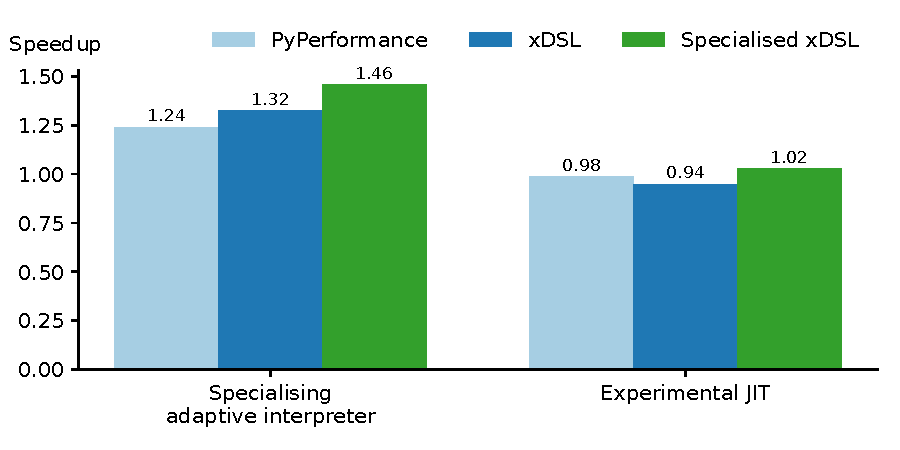
\includegraphics[width=0.75\textwidth]{images/impact_cpython_optimisations/15_summary.pdf}
    \caption{Highly dynamic workloads such as constant folding in xDSL exacerbate the performance impact of CPython optimisations leveraging runtime information, with manual specialisation further revealing optimisation opportunities.}
    \label{figure:impact-cpython-optimisations}
\end{figure}



This can be seen by constant folding in xDSL having a greater speedup than PyPerformance with the specialising adaptive interpreter, but a worse slow-down with the experimental \ac{jit}.
In addition to this, we show that specialisation of the workloads (\autoref{chap:specialising-optimising-pattern-rewriting}) reveals further optimisation opportunities, increasing the impact of both of these dynamic optimisations.







% This is interesting, but needs more writing/word count and is unrelated to the narrative of dynamism

% \section{Tail call interpreter}
% \label{sec:tail-call-interpreter}

% %% Motivation
% % Hook
% In addition to \ac{jit} optimisations leveraging runtime information, there are other opportunities for improving the implementation of interpreted runtimes.
% % Argument
% Interpreters can be modelled as a loop which iterates through a sequence of bytecode instructions, with a switch statement selecting the evaluation logic at each iteration for the current instruction.
% This leads to challenges \cite{mikepallReSuggestionsImplementing2011}.
% In addition to their work on copy-and-patch compilation, Haoran Xu's work on interpreted language runtimes introduces another idea to address this problem. Tail calling interpreters
% \cite{xuDeegenJITCapableVM2024}
% % Link
% This concept has recently been included in the most recent CPython minor version release, 3.14, with the final release version expected in November 2025.

% %% How is it implemented?
% % Hook
% % Argument
% % Implementation details
% % Overall performance speedup (cited, ours recorded)
% % How does this relate to dynamism
% % Link
% As with the previous two approaches, we substantiate these claims by an ablation of the feature across the previously discussed real-world workload and micro-benchmarks (\autoref{tab:tail-call-interpreter-xdsl}).

% \begin{table}[H]
%   \caption{.}
%   \label{tab:tail-call-interpreter-xdsl}
%   \centering
%   \begin{tabular}{lllc}
%     \toprule
%     & \multicolumn{2}{c}{\textbf{Execution time [ns]}} \\
%     \cmidrule(r){2-3}
%     \textbf{Workload}& \textbf{Baseline} & \textbf{Optimised} & \textbf{Speedup} \\
%     \midrule
%     Operation traversal & \\
%     Trait checking & \\
%     Operation instantiation & \\
%     % ...
%     Constant folding & \\
%     \bottomrule
%   \end{tabular}
% \end{table}

% %% How does it perform in xDSL??
% % Hook
% % Argument
% % Link
